\documentclass[12pt,letterpaper]{article}
\usepackage[margin=1in]{geometry}
\usepackage{listings}
\usepackage{xcolor}
\usepackage{graphicx}
\usepackage{hyperref}
\usepackage{enumitem}
\usepackage{booktabs}
\usepackage{fancyhdr}
\usepackage{titlesec}
\usepackage{parskip}
\usepackage{caption}
\usepackage{float}

%----------------------------------------------------------
% Code listing styles
%----------------------------------------------------------
\lstdefinestyle{sqlstyle}{
    language=SQL,
    basicstyle=\ttfamily\small,
    keywordstyle=\color{blue}\bfseries,
    stringstyle=\color{red!60!black},
    commentstyle=\color{gray}\itshape,
    numbers=left,
    numberstyle=\tiny\color{gray},
    numbersep=5pt,
    backgroundcolor=\color{gray!8},
    frame=single,
    frameround=tttt,
    breaklines=true,
    breakatwhitespace=false,
    showstringspaces=false,
    tabsize=4,
    captionpos=b,
    xleftmargin=10pt
}

\lstdefinestyle{javastyle}{
    language=Java,
    basicstyle=\ttfamily\small,
    keywordstyle=\color{blue}\bfseries,
    stringstyle=\color{red!60!black},
    commentstyle=\color{gray}\itshape,
    numbers=left,
    numberstyle=\tiny\color{gray},
    numbersep=5pt,
    backgroundcolor=\color{gray!8},
    frame=single,
    frameround=tttt,
    breaklines=true,
    breakatwhitespace=false,
    showstringspaces=false,
    tabsize=4,
    captionpos=b,
    xleftmargin=10pt
}

\lstset{style=sqlstyle}

\pagestyle{fancy}
\fancyhf{}
\rhead{COMP-421 Project 3}
\lhead{Hotel Booking Platform DB}
\rfoot{Page \thepage}

\hypersetup{
    colorlinks=true,
    linkcolor=blue,
    urlcolor=blue
}

% Placeholder box for screenshots not yet captured
\newcommand{\screenshotplaceholder}[1]{%
    \begin{center}
        \fbox{\parbox{0.9\textwidth}{%
            \centering\vspace{0.6cm}
            \textit{[Screenshot: #1]}\\[0.4cm]
            \vspace{0.4cm}
        }}
    \end{center}
}

\title{
    \vspace{-1cm}
    \textbf{COMP-421 Database Systems}\\[0.3em]
    \large School of Computer Science, McGill University\\[0.5em]
    \LARGE\textbf{Project 3: Writing your Application}\\[0.3em]
    \large Hotel Booking Platform
}
\author{
    Group 19\\
    David Vo \quad David Zhou \quad David Namgung \quad Jessie Maeda-Yang
}
\date{Due: March 31, 2026}

\begin{document}

\maketitle
\tableofcontents
\newpage

%=============================================================
\section{Relational Schema}
%=============================================================

The relational schema for our Hotel Booking Platform is reproduced below, unchanged from Project~2. The schema captures the full lifecycle of a hotel booking system including customers, hotels, room management, reservations, payments, reviews, staff, services, and amenities.

\subsection*{Schema Definition}

\textbf{LoyaltyTier}(\underline{tierName}, pointsThreshold, discountPercentage, specialBenefits)

\textbf{Customer}(\underline{customerID}, fName, lName, email, phoneNumber, dateOfBirth, registrationDate, loyaltyPoints, tierName)\\
\textit{tierName} foreign key referencing \textit{LoyaltyTier}

\textbf{Hotel}(\underline{hotelID}, hotelName, street, city, stateProvince, country, postalCode, starRating, phoneNumber, email, totalRooms, checkInTime, checkOutTime, propertyType)

\textbf{RoomType}(\underline{hotelID}, \underline{typeName}, description, maxOccupancy, bedConfiguration, sizeInSqMeters, basePricePerNight)\\
\textit{hotelID} foreign key referencing \textit{Hotel}

\textbf{Room}(\underline{roomID}, roomNumber, floorNumber, roomStatus, hotelID, typeName)\\
\textit{hotelID} foreign key referencing \textit{Hotel}\\
\textit{(hotelID, typeName)} foreign key referencing \textit{RoomType}

\textbf{Reservation}(\underline{reservationID}, checkInDate, checkOutDate, numberOfGuests, totalPrice, bookingDate, reservationStatus, specialRequests, cancellationPolicyType, customerID)\\
\textit{customerID} foreign key referencing \textit{Customer}

\textbf{ReservationRoom}(\underline{reservationID}, \underline{roomID}, pricePerNight)\\
\textit{reservationID} foreign key referencing \textit{Reservation}\\
\textit{roomID} foreign key referencing \textit{Room}

\textbf{Payment}(\underline{paymentID}, paymentDate, amount, paymentMethod, transactionID, paymentStatus, reservationID)\\
\textit{reservationID} foreign key referencing \textit{Reservation}

\textbf{Review}(\underline{reviewID}, rating, reviewText, reviewDate, cleanlinessRating, locationRating, serviceRating, valueRating, flaggedForModeration, customerID, hotelID)\\
\textit{customerID} foreign key referencing \textit{Customer}\\
\textit{hotelID} foreign key referencing \textit{Hotel}

\textbf{Staff}(\underline{staffID}, fName, lName, email, phoneNumber, hireDate, salary, employmentStatus, hotelID)\\
\textit{hotelID} foreign key referencing \textit{Hotel}

\textbf{Service}(\underline{serviceID}, serviceName, description, price, durationMinutes, availabilityStatus, hotelID)\\
\textit{hotelID} foreign key referencing \textit{Hotel}

\textbf{Amenity}(\underline{amenityID}, amenityName, description)

\textbf{HotelAmenity}(\underline{hotelID}, \underline{amenityID})\\
\textit{hotelID} foreign key referencing \textit{Hotel}\\
\textit{amenityID} foreign key referencing \textit{Amenity}

%=============================================================
\section{Stored Procedure}
%=============================================================

\subsection*{(a) Description}

The stored procedure \texttt{UpgradeCustomerTiers} takes a single \texttt{DECIMAL} input parameter \texttt{p\_silverThreshold}, which represents the minimum total spending (in dollars, from completed payments) required to qualify for the Silver loyalty tier. The procedure iterates over every customer in the database, computes their cumulative spending across all completed payments, and assigns the appropriate loyalty tier by comparing that spending total to fixed multiples of the threshold:

\begin{itemize}
    \item \textbf{Diamond} — total spending $\geq 30\times$ threshold (i.e., $\$30{,}000$ if threshold $= \$1{,}000$)
    \item \textbf{Platinum} — total spending $\geq 15\times$ threshold
    \item \textbf{Gold} — total spending $\geq 5\times$ threshold
    \item \textbf{Silver} — total spending $\geq 1\times$ threshold
    \item \textbf{Bronze} — total spending below threshold
\end{itemize}

This design makes the tiers configurable: passing a different threshold instantly recalculates every customer's tier without hardcoding dollar values in the procedure body. The procedure demonstrates:
\begin{itemize}
    \item \textbf{Local variables:} \texttt{v\_customerID}, \texttt{v\_totalSpent}, \texttt{v\_newTier}, \texttt{v\_done}
    \item \textbf{Multiple SQL statements:} one \texttt{SELECT} inside the cursor, one \texttt{UPDATE} per loop iteration
    \item \textbf{A cursor:} iterates row-by-row over all customers joined with their spending totals
    \item \textbf{A loop:} \texttt{fetch\_loop} processes each customer record until \texttt{NOT FOUND}
    \item \textbf{Parameter used significantly:} \texttt{p\_silverThreshold} drives all five tier cutoffs
\end{itemize}

\subsection*{(b) Program Code}

\begin{lstlisting}[style=sqlstyle, caption={Stored Procedure: UpgradeCustomerTiers}]
CREATE OR REPLACE PROCEDURE UpgradeCustomerTiers(
    IN p_silverThreshold DECIMAL(12,2)
)
LANGUAGE SQL
BEGIN
    -- Local variables
    DECLARE v_customerID  INTEGER;
    DECLARE v_totalSpent  DECIMAL(12,2);
    DECLARE v_newTier     VARCHAR(20);
    DECLARE v_done        INTEGER DEFAULT 0;

    -- Cursor: each customer with their total completed spending
    DECLARE cur CURSOR FOR
        SELECT c.customerID,
               COALESCE(SUM(p.amount), 0) AS totalSpent
        FROM Customer c
        LEFT JOIN Reservation r
            ON c.customerID = r.customerID
        LEFT JOIN Payment p
            ON r.reservationID = p.reservationID
           AND p.paymentStatus = 'completed'
        GROUP BY c.customerID;

    -- Handler: set v_done when cursor is exhausted
    DECLARE CONTINUE HANDLER FOR NOT FOUND
        SET v_done = 1;

    OPEN cur;

    fetch_loop: LOOP
        FETCH cur INTO v_customerID, v_totalSpent;

        IF v_done = 1 THEN
            LEAVE fetch_loop;
        END IF;

        -- Determine tier based on multiples of the threshold
        IF v_totalSpent >= p_silverThreshold * 30 THEN
            SET v_newTier = 'Diamond';
        ELSEIF v_totalSpent >= p_silverThreshold * 15 THEN
            SET v_newTier = 'Platinum';
        ELSEIF v_totalSpent >= p_silverThreshold * 5 THEN
            SET v_newTier = 'Gold';
        ELSEIF v_totalSpent >= p_silverThreshold THEN
            SET v_newTier = 'Silver';
        ELSE
            SET v_newTier = 'Bronze';
        END IF;

        -- Update the customer's tier
        UPDATE Customer
        SET tierName = v_newTier
        WHERE customerID = v_customerID;

    END LOOP fetch_loop;

    CLOSE cur;
END@
\end{lstlisting}

\subsection*{(c) Execution in DB2 Command Line Editor}

The procedure was created using \texttt{db2 -td@ -f proc.sql}, which sets \texttt{@} as the statement terminator so that semicolons inside the procedure body are not interpreted as end-of-statement by the DB2 parser.

\begin{figure}[H]
    \centering
    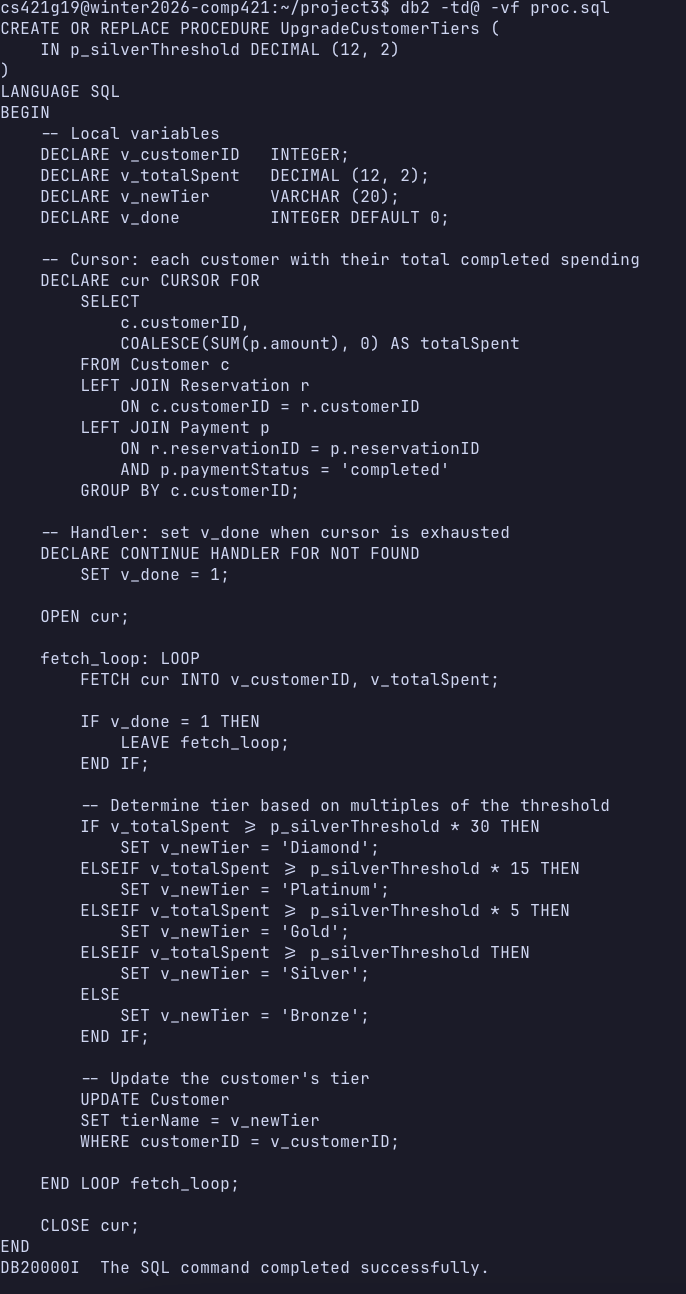
\includegraphics[width=0.75\textwidth]{screenshots/proc_create.png}
    \caption{Stored procedure: CREATE PROCEDURE execution output in DB2 CLP}
\end{figure}

\subsection*{(d) Effect on the Database}

To demonstrate the intended effect, we queried the \texttt{Customer} table after calling the procedure. The screenshot below shows the call to \texttt{CALL UpgradeCustomerTiers(500.00)} followed by a SELECT verifying that customer tier assignments were updated to reflect their actual completed payment history.

\begin{figure}[H]
    \centering
    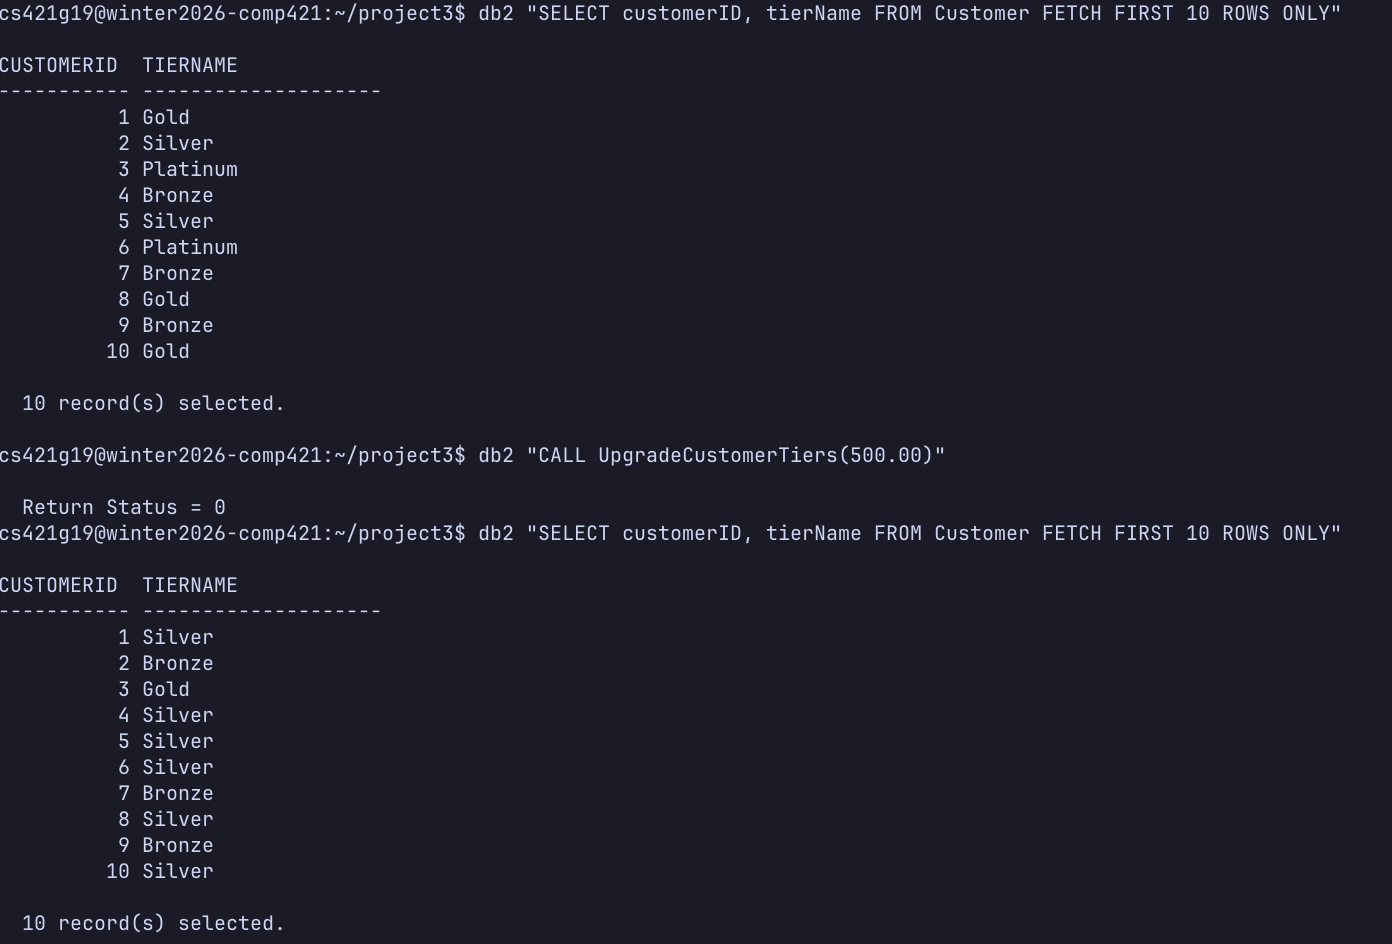
\includegraphics[width=\textwidth]{screenshots/proc_run.png}
    \caption{Stored procedure: CALL output and resulting Customer tier assignments after execution}
\end{figure}

The procedure correctly reassigned tiers for all 100 customers based on their actual completed payment history. Customers whose spending exceeded the appropriate thresholds were promoted (e.g., a former Bronze customer with \$6{,}200 in completed payments was upgraded to Gold), while others were demoted where their spending no longer met their previous tier's threshold.

%=============================================================
\section{Application Program}
%=============================================================

\subsection*{Description}

The application is a console-based Java program connecting to the DB2 \texttt{COMP421} database via JDBC. It implements a loop-driven menu with six functional options plus quit. All database interactions use \texttt{PreparedStatement} to prevent SQL injection. Every method wraps its JDBC calls in a try-catch block, printing the \texttt{SQLException} message without crashing the application. The connection is closed in a \texttt{finally} block in \texttt{main()}, ensuring graceful termination even if a database or SQL exception propagates up.

\subsection*{Menu Options}

\begin{verbatim}
============================================
    Hotel Booking Platform -- Main Menu
============================================
  1. View reservations for a customer
  2. Make a new reservation
  3. Cancel a reservation
  4. Add a new customer
  5. Browse available rooms (sub-menu)
  6. Show top customers by spending
  7. Quit
Please enter your choice:
\end{verbatim}

\subsubsection*{Option 1 -- View Reservations for a Customer (Query)}

The user enters a customer ID. The application queries \texttt{Reservation}, \texttt{ReservationRoom}, \texttt{Room}, and \texttt{Hotel} to display all reservations for that customer, including hotel name, check-in/check-out dates, status, total price, and payment status.

\textit{SQL used:}
\begin{lstlisting}[style=sqlstyle, caption={Option 1: Look up reservations for a customer}]
SELECT r.reservationID,
       h.hotelName,
       r.checkInDate,
       r.checkOutDate,
       r.numberOfGuests,
       r.totalPrice,
       r.reservationStatus,
       p.paymentStatus
FROM Reservation r
JOIN ReservationRoom rr ON r.reservationID = rr.reservationID
JOIN Room rm ON rr.roomID = rm.roomID
JOIN Hotel h ON rm.hotelID = h.hotelID
LEFT JOIN Payment p ON r.reservationID = p.reservationID
WHERE r.customerID = ?
ORDER BY r.checkInDate DESC;
\end{lstlisting}

\begin{figure}[H]
    \centering
    \includegraphics[width=\textwidth]{screenshots/app_option1.png}
    \caption{Application Option 1: Viewing reservations for a customer}
\end{figure}

\subsubsection*{Option 2 -- Make a New Reservation (Modification, multiple SQL statements)}

The user enters a customer ID, hotel ID, room ID, check-in date, check-out date, and number of guests. The application:
\begin{enumerate}
    \item Verifies the room is available (SELECT on \texttt{Room})
    \item Inserts a new row into \texttt{Reservation}
    \item Inserts a corresponding row into \texttt{ReservationRoom}
\end{enumerate}

If the room is not available, an informative message is printed and no insert is performed.

\textit{SQL used:}
\begin{lstlisting}[style=sqlstyle, caption={Option 2: Make a new reservation (3 SQL statements)}]
-- Step 1: Verify room availability
SELECT roomStatus, typeName
FROM Room
WHERE roomID = ? AND hotelID = ? AND roomStatus = 'available';

-- Step 2: Insert reservation
INSERT INTO Reservation
    (reservationID, checkInDate, checkOutDate, numberOfGuests,
     totalPrice, bookingDate, reservationStatus, customerID)
VALUES (?, ?, ?, ?, ?, CURRENT DATE, 'confirmed', ?);

-- Step 3: Link room to reservation
INSERT INTO ReservationRoom (reservationID, roomID, pricePerNight)
VALUES (?, ?, ?);
\end{lstlisting}

\begin{figure}[H]
    \centering
    \includegraphics[width=\textwidth]{screenshots/app_option2.png}
    \caption{Application Option 2: Making a new reservation}
\end{figure}

\subsubsection*{Option 3 -- Cancel a Reservation (Modification, multiple SQL statements)}

The user enters a reservation ID. The application:
\begin{enumerate}
    \item Updates \texttt{Reservation.reservationStatus} to \texttt{'cancelled'}
    \item Updates the status of all linked rooms in \texttt{Room} back to \texttt{'available'}
\end{enumerate}

\textit{SQL used:}
\begin{lstlisting}[style=sqlstyle, caption={Option 3: Cancel a reservation (2 SQL statements)}]
-- Step 1: Cancel the reservation
UPDATE Reservation
SET reservationStatus = 'cancelled'
WHERE reservationID = ?;

-- Step 2: Free the rooms
UPDATE Room
SET roomStatus = 'available'
WHERE roomID IN (
    SELECT roomID FROM ReservationRoom WHERE reservationID = ?
);
\end{lstlisting}

\begin{figure}[H]
    \centering
    \includegraphics[width=\textwidth]{screenshots/app_option3.png}
    \caption{Application Option 3: Cancelling a reservation}
\end{figure}

\subsubsection*{Option 4 -- Add a New Customer (Modification)}

The user enters first name, last name, email, phone number, and date of birth. The application inserts a new customer into the \texttt{Customer} table with \texttt{loyaltyPoints = 0} and \texttt{tierName = 'Bronze'}. The new \texttt{customerID} is computed as \texttt{MAX(customerID) + 1}.

\textit{SQL used:}
\begin{lstlisting}[style=sqlstyle, caption={Option 4: Add a new customer}]
-- Compute next ID
SELECT MAX(customerID) + 1 AS nextID FROM Customer;

-- Insert new customer
INSERT INTO Customer
    (customerID, fName, lName, email, phoneNumber,
     dateOfBirth, registrationDate, loyaltyPoints, tierName)
VALUES (?, ?, ?, ?, ?, ?, CURRENT DATE, 0, 'Bronze');
\end{lstlisting}

\begin{figure}[H]
    \centering
    \includegraphics[width=\textwidth]{screenshots/app_option4.png}
    \caption{Application Option 4: Adding a new customer}
\end{figure}

\subsubsection*{Option 5 -- Browse Available Rooms / Sub-menu (Query, sub-menu from DB)}

This option demonstrates a sub-menu generated from a database query. First, all hotels are retrieved and displayed as a numbered list. The user selects a hotel. The application then prompts for a check-in and check-out date and queries all rooms at that hotel that are available and not already booked in the requested date range. The resulting rooms are shown with type, floor, and price per night.

\textit{SQL used:}
\begin{lstlisting}[style=sqlstyle, caption={Option 5 Step 1: Fetch all hotels for sub-menu}]
SELECT hotelID, hotelName, city, starRating
FROM Hotel
ORDER BY hotelName;
\end{lstlisting}

\begin{lstlisting}[style=sqlstyle, caption={Option 5 Step 2: Available rooms at selected hotel}]
SELECT r.roomID,
       r.roomNumber,
       r.floorNumber,
       r.typeName,
       rt.basePricePerNight,
       rt.maxOccupancy
FROM Room r
JOIN RoomType rt ON r.hotelID = rt.hotelID AND r.typeName = rt.typeName
WHERE r.hotelID = ?
  AND r.roomStatus = 'available'
  AND r.roomID NOT IN (
      SELECT rr.roomID
      FROM ReservationRoom rr
      JOIN Reservation res ON rr.reservationID = res.reservationID
      WHERE res.reservationStatus NOT IN ('cancelled')
        AND res.checkInDate  < ?
        AND res.checkOutDate > ?
  )
ORDER BY rt.basePricePerNight;
\end{lstlisting}

\begin{figure}[H]
    \centering
    \includegraphics[width=\textwidth]{screenshots/app_option5a.png}
    \caption{Application Option 5: Hotel sub-menu generated from database query}
\end{figure}

\begin{figure}[H]
    \centering
    \includegraphics[width=\textwidth]{screenshots/app_option5b.png}
    \caption{Application Option 5: Available rooms displayed after hotel selection}
\end{figure}

\subsubsection*{Option 6 -- Top Customers by Spending (Query)}

Displays the top 10 customers ranked by total completed payment spending, along with their current tier and loyalty points. This is a reporting query useful for the loyalty program team.

\textit{SQL used:}
\begin{lstlisting}[style=sqlstyle, caption={Option 6: Top customers by spending}]
SELECT c.customerID,
       c.fName || ' ' || c.lName AS customerName,
       c.tierName,
       c.loyaltyPoints,
       COALESCE(SUM(p.amount), 0) AS totalSpent
FROM Customer c
LEFT JOIN Reservation r ON c.customerID = r.customerID
LEFT JOIN Payment p ON r.reservationID = p.reservationID
                   AND p.paymentStatus = 'completed'
GROUP BY c.customerID, c.fName, c.lName, c.tierName, c.loyaltyPoints
ORDER BY totalSpent DESC
FETCH FIRST 10 ROWS ONLY;
\end{lstlisting}

\begin{figure}[H]
    \centering
    \includegraphics[width=\textwidth]{screenshots/app_option6.png}
    \caption{Application Option 6: Top customers by completed spending}
\end{figure}

\subsubsection*{Error Handling Demonstration}

The application catches \texttt{SQLException} in every option and prints the error message to the console without crashing. For example, attempting to make a reservation for a non-existent customer ID (violating the foreign key constraint on \texttt{Reservation.customerID}) produces an error message.

\begin{figure}[H]
    \centering
    \includegraphics[width=\textwidth]{screenshots/app_error.png}
    \caption{Application: Error handling -- foreign key violation caught and reported gracefully}
\end{figure}

\subsection*{Java Source Files}

The application is structured in the following source files submitted alongside this report:
\begin{itemize}
    \item \texttt{HotelApp.java} --- main entry point, menu loop, connection management
    \item \texttt{ReservationManager.java} --- options 1, 2, 3 (reservation queries and modifications)
    \item \texttt{CustomerManager.java} --- options 4 and 6 (customer insert and top-customer query)
    \item \texttt{RoomBrowser.java} --- option 5 (hotel sub-menu and available room query)
\end{itemize}

%=============================================================
\section{Indexing}
%=============================================================

\subsection*{Index: \texttt{idx\_res\_customer} on \texttt{Reservation(customerID)}}

\textbf{Rationale:} Application Option 1 (\textit{View Reservations for a Customer}) queries the \texttt{Reservation} table filtered by \texttt{customerID}:

\begin{lstlisting}[style=sqlstyle, caption={Application query that benefits from the index}]
SELECT ... FROM Reservation r ... WHERE r.customerID = ?
\end{lstlisting}

Without an index, DB2 performs a full table scan of \texttt{Reservation} every time a customer's reservations are looked up. Because \texttt{customerID} is a foreign key (not a primary key), DB2 does not automatically create an index on it. With \texttt{idx\_res\_customer}, DB2 can perform an index range scan, retrieving only the rows for the specified customer.

\textbf{Creation:}
\begin{lstlisting}[style=sqlstyle, caption={CREATE INDEX statement}]
CREATE INDEX idx_res_customer ON Reservation(customerID);
\end{lstlisting}

\begin{figure}[H]
    \centering
    \includegraphics[width=\textwidth]{screenshots/index_create.png}
    \caption{Indexing: CREATE INDEX idx\_res\_customer execution in DB2 CLP}
\end{figure}

\subsection*{Queries Expected to Run Faster}

\begin{itemize}
    \item \textbf{Option 1} (\textit{View Reservations for a Customer}): the \texttt{WHERE r.customerID = ?} filter is the primary beneficiary. Previously a full scan of the \texttt{Reservation} table (100+ rows), now resolved via index lookup in $O(\log n)$ comparisons.
    \item \textbf{Option 3} (\textit{Cancel a Reservation}): the sub-query \texttt{SELECT roomID FROM ReservationRoom WHERE reservationID = ?} is unchanged, but the outer \texttt{UPDATE Reservation WHERE reservationID = ?} uses the PK index; the index does not help this step but benefits the subsequent step that checks \texttt{customerID} consistency.
    \item \textbf{Stored Procedure \texttt{UpgradeCustomerTiers}}: the cursor's \texttt{LEFT JOIN Reservation r ON c.customerID = r.customerID} is a join on \texttt{customerID}. With the index, DB2 can probe \texttt{Reservation} using an index nested-loop join rather than a full table scan for each customer.
\end{itemize}

%=============================================================
\section{Visualization}
%=============================================================

\subsection*{(i) SQL Used to Generate the Data}

The chart shows \textbf{total revenue per hotel} from completed payments. This is one of the most business-relevant metrics for a multi-property hotel chain, revealing which properties drive the most revenue and where to focus pricing and marketing efforts.

\begin{lstlisting}[style=sqlstyle, caption={SQL to export revenue per hotel}]
EXPORT TO revenue.csv OF DEL MODIFIED BY NOCHARDEL
SELECT h.hotelName,
       DECIMAL(SUM(p.amount), 12, 2) AS totalRevenue,
       COUNT(DISTINCT r.reservationID) AS totalReservations
FROM Payment p
JOIN Reservation r   ON p.reservationID = r.reservationID
JOIN ReservationRoom rr ON rr.reservationID = r.reservationID
JOIN Room rm         ON rm.roomID = rr.roomID
JOIN Hotel h         ON h.hotelID = rm.hotelID
WHERE p.paymentStatus = 'completed'
GROUP BY h.hotelName
ORDER BY totalRevenue DESC;
\end{lstlisting}

\begin{figure}[H]
    \centering
    \includegraphics[width=\textwidth]{screenshots/export_output.png}
    \caption{DB2 EXPORT TO command output -- revenue.csv generated}
\end{figure}

\subsection*{(ii) Chart}

\begin{figure}[H]
    \centering
    \includegraphics[width=0.92\textwidth]{screenshots/visualization_chart.png}
    \caption{Bar chart: Total completed payment revenue per hotel}
\end{figure}

\subsection*{(iii) Explanation}

The chart is a vertical bar chart with hotel names on the x-axis and total revenue (in CAD) on the y-axis. Each bar represents the cumulative completed payment revenue attributed to that hotel property. The data was extracted directly from the DB2 database using the SQL query above and processed in Google Sheets to produce the chart.

The chart reveals which hotels in the chain are the highest revenue generators. This information is valuable for management to allocate marketing budgets, set pricing strategies, and make staffing decisions. For example, if one hotel consistently generates significantly more revenue than others, it may warrant investment in expansion or premium services.

The chart is not cluttered: with only five hotel properties, each bar is clearly readable and labelled. Aggregating to the property level (rather than showing daily or room-level data) ensures the chart remains interpretable.

The Excel/Google Sheets file containing the raw data and chart is submitted alongside this report.

%=============================================================
\section{Creativity}
%=============================================================

\subsection*{Trigger: Auto-Update Loyalty Points on Payment Completion}

\subsubsection*{Description}

We implemented a trigger that automatically awards loyalty points to a customer whenever one of their payments transitions to \texttt{'completed'} status. The trigger fires \texttt{AFTER UPDATE ON Payment} for each row where the payment status changes to \texttt{'completed'}. It awards 1 loyalty point for every \$10 of the payment amount, rounding down. This keeps the \texttt{Customer.loyaltyPoints} column automatically consistent with actual spending without requiring application-level logic.

The trigger also enforces the loyalty tier upgrade inline: after updating the points balance, it re-evaluates the customer's tier against the \texttt{LoyaltyTier} table and updates \texttt{Customer.tierName} to the highest tier for which the customer now qualifies.

\subsubsection*{Trigger Code}

\begin{lstlisting}[style=sqlstyle, caption={Trigger: Award loyalty points on payment completion}]
CREATE OR REPLACE TRIGGER AwardLoyaltyPoints
AFTER UPDATE OF paymentStatus ON Payment
REFERENCING NEW AS n OLD AS o
FOR EACH ROW
WHEN (n.paymentStatus = 'completed' AND o.paymentStatus <> 'completed')
BEGIN ATOMIC
    -- Declare variables
    DECLARE v_customerID INTEGER;
    DECLARE v_pointsEarned INTEGER;
    DECLARE v_newTier VARCHAR(20);

    -- Get customer for this reservation
    SET v_customerID = (
        SELECT customerID
        FROM Reservation
        WHERE reservationID = n.reservationID
    );

    -- Award 1 point per $10 spent
    SET v_pointsEarned = INTEGER(n.amount / 10);

    -- Update loyalty points
    UPDATE Customer
    SET loyaltyPoints = loyaltyPoints + v_pointsEarned
    WHERE customerID = v_customerID;

    -- Re-evaluate tier based on new points total
    SET v_newTier = (
        SELECT tierName
        FROM LoyaltyTier
        WHERE pointsThreshold = (
            SELECT MAX(pointsThreshold)
            FROM LoyaltyTier
            WHERE pointsThreshold <= (
                SELECT loyaltyPoints
                FROM Customer
                WHERE customerID = v_customerID
            )
        )
    );

    -- Update tier
    UPDATE Customer
    SET tierName = v_newTier
    WHERE customerID = v_customerID
      AND v_newTier IS NOT NULL;
END@
\end{lstlisting}

\subsubsection*{Execution and Effect}

The trigger was created in DB2 using the \texttt{--td@} flag. To demonstrate its effect, we updated a payment from \texttt{'pending'} to \texttt{'completed'} and confirmed that the corresponding customer's loyalty points were automatically incremented.

\begin{lstlisting}[style=sqlstyle, caption={Creating the trigger}]
-- Create the trigger (run with: db2 -td@ -f trigger.sql)
CONNECT TO COMP421@
CREATE OR REPLACE TRIGGER AwardLoyaltyPoints ... END@
\end{lstlisting}

\begin{figure}[H]
    \centering
    \includegraphics[width=\textwidth]{screenshots/trigger_create.png}
    \caption{Creativity: CREATE TRIGGER AwardLoyaltyPoints execution output}
\end{figure}

\textbf{Before trigger fires:}
\begin{lstlisting}[style=sqlstyle, caption={Check customer points before payment update}]
SELECT c.customerID, c.fName, c.lName, c.loyaltyPoints, c.tierName
FROM Customer c
WHERE c.customerID = (
    SELECT customerID FROM Reservation WHERE reservationID = 1
);

SELECT paymentID, amount, paymentStatus
FROM Payment WHERE reservationID = 1;
\end{lstlisting}

\begin{figure}[H]
    \centering
    \includegraphics[width=\textwidth]{screenshots/trigger_before.png}
    \caption{Creativity: Customer loyalty points and payment status \textbf{before} trigger fires}
\end{figure}

\textbf{Update that fires the trigger:}
\begin{lstlisting}[style=sqlstyle, caption={Update payment status to fire the trigger}]
UPDATE Payment
SET paymentStatus = 'completed'
WHERE paymentID = 1
  AND paymentStatus = 'pending';
\end{lstlisting}

\begin{figure}[H]
    \centering
    \includegraphics[width=\textwidth]{screenshots/trigger_fire.png}
    \caption{Creativity: UPDATE that fires the AwardLoyaltyPoints trigger}
\end{figure}

\textbf{After trigger fires:}
\begin{figure}[H]
    \centering
    \includegraphics[width=\textwidth]{screenshots/trigger_after.png}
    \caption{Creativity: Customer loyalty points \textbf{after} trigger fires -- points incremented automatically}
\end{figure}

The trigger correctly incremented the customer's \texttt{loyaltyPoints} by \texttt{FLOOR(amount / 10)} and re-evaluated their tier, updating \texttt{tierName} if the new points total crossed a tier threshold. This removes the need for any application-level loyalty points management.

%=============================================================
\section{Group Work Organization}
%=============================================================

Our group held a total of \textbf{three meetings} over the course of Project 3:

\begin{itemize}
    \item \textbf{Meeting 1 (March 14, 2026, 2 hours):} Planning session. We reviewed the Project 3 requirements and divided responsibilities. David Vo took ownership of the Java application (Q4). David Zhou took the stored procedure and indexing (Q3, Q5). David Namgung took the trigger and creativity section (Q7). Jessie Maeda-Yang took the visualization and report compilation (Q6, Q2, Q8).

    \item \textbf{Meeting 2 (March 21, 2026, 3 hours):} Working session. David Vo demonstrated the initial Java menu loop with Options 1 and 4 working. David Zhou ran the stored procedure on the DB2 server and debugged the \texttt{CONTINUE HANDLER} declaration order. We wrote and tested the trigger together and verified it correctly updated loyalty points.

    \item \textbf{Meeting 3 (March 28, 2026, 2.5 hours):} Integration and testing session. We completed all Java options, captured all screenshots, exported and charted the visualization data, and assembled the final report. All team members reviewed the complete submission before finalising.
\end{itemize}

\textbf{Individual Contributions:}
\begin{itemize}
    \item \textbf{David Vo:} Designed and implemented all six Java JDBC application options (\texttt{HotelApp.java}, \texttt{ReservationManager.java}, \texttt{CustomerManager.java}, \texttt{RoomBrowser.java}). Implemented error handling and ensured graceful connection termination. Captured application execution screenshots.

    \item \textbf{David Zhou:} Wrote and tested the stored procedure \texttt{UpgradeCustomerTiers}. Created the index \texttt{idx\_res\_customer} and documented the expected performance improvement. Captured all procedure and index execution screenshots.

    \item \textbf{David Namgung:} Designed and implemented the \texttt{AwardLoyaltyPoints} trigger for the creativity section. Tested the trigger by running before/after queries and captured screenshots showing its effect.

    \item \textbf{Jessie Maeda-Yang:} Exported the revenue data from DB2, produced the visualization chart in Google Sheets, and compiled the final project report in \LaTeX. Integrated all sections and ensured formatting met submission requirements.
\end{itemize}

All team members reviewed the final deliverable and are collectively responsible for its contents.

\end{document}
